\begin{align*}
    \polynomialQ{1}{X}{0} &= 0 \\
    \polynomialQ{1}{X}{1} &= 1 \\
    \polynomialQ{1}{X}{2} &= 6X - 4 \\
    \polynomialQ{1}{X}{3} &= 18X - 27 \\
    \polynomialQ{1}{X}{4} &= 36X - 80 \\
    \polynomialQ{1}{X}{5} &= 60X - 175 \\
    \polynomialQ{1}{X}{6} &= 90X - 324 \\
    \polynomialQ{1}{X}{7} &= 126X - 539 \\
    \polynomialQ{1}{X}{8} &= 168X - 832 \\
    \polynomialQ{1}{X}{9} &= 216X - 1215 \\
    \polynomialQ{1}{X}{10} &= 270X - 1700 \\
    \polynomialQ{1}{X}{11} &= 330X - 2299 \\
    \polynomialQ{1}{X}{12} &= 396X - 3024 \\
    \polynomialQ{1}{X}{13} &= 468X - 3887 \\
    \polynomialQ{1}{X}{14} &= 546X - 4900 \\
    \polynomialQ{1}{X}{15} &= 630X - 6075 \\
    \polynomialQ{1}{X}{16} &= 720X - 7424 \\
    \polynomialQ{1}{X}{17} &= 816X - 8959 \\
    \polynomialQ{1}{X}{18} &= 918X - 10692 \\
    \polynomialQ{1}{X}{19} &= 1026X - 12635 \\
    \polynomialQ{1}{X}{20} &= 1140X - 14800
\end{align*}
\begin{figure}[H]
    \centering
    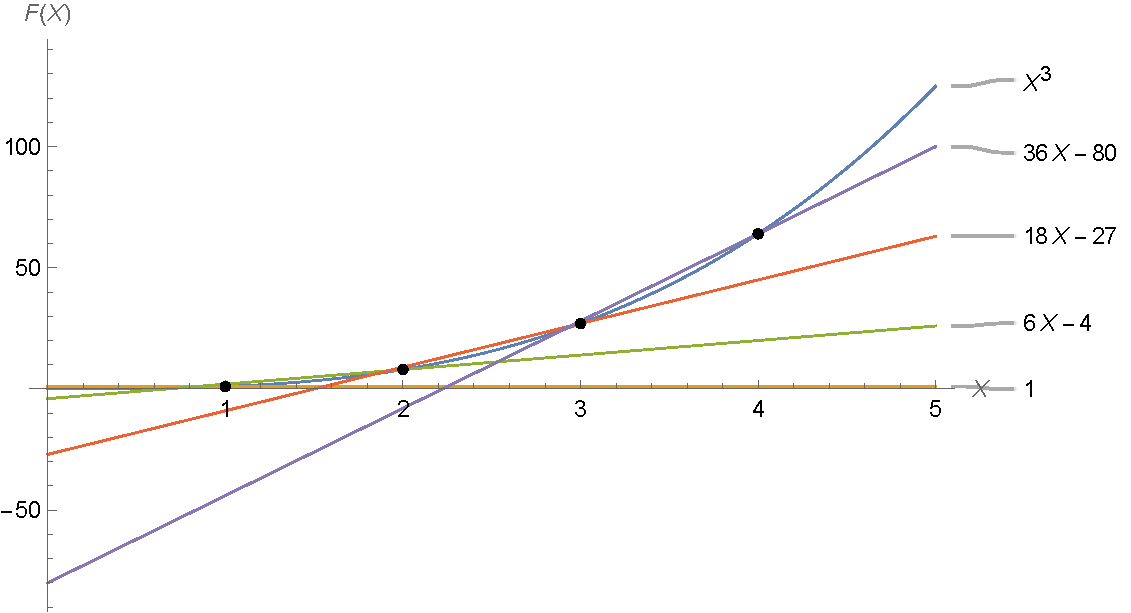
\includegraphics[width=1\textwidth]{sections/images/02_cubes_with_q_1_n_k}
    ~\caption{Polynomials Q(1, n, k)}\label{fig:figure2}
\end{figure}

